%!TEX root = ../Tibt.tex

\exercise{3.2}

\seecode

The premise of the two confidence band estimates is that the posterior
distribution of the true value $\beta$ given the data is that of a gaussian vector, 
with center $\hat{\beta}$ and covariance $ \hat{\sigma}^2 \left( \mathbf{X} ^T \mathbf{X}  \right) ^{-1}$. In the case described by the exercise $\mathbf{X}$
is the matrix whose columns contains increasing powers of the samples of $X$.
The two confidence bands are then obtained as follows:
\begin{enumerate}
    \item Since $\beta^T x_0$ is also gaussian with mean $\hat{y}_0 \equiv \hat{\beta}^T x_0$ and variance $\hat{\sigma}^2\, x_0^T ( \mathbf{X} ^T \mathbf{X})^{-1} x_0$, we can define a confidence band for its value via:
    \begin{eqnarray*}
        \mathcal{C}_1 =  \left\{ y \; : \; (y - \hat{y}_0)^2 \leq \hat{\sigma}^2 \, x_0^T ( \mathbf{X} ^T \mathbf{X})^{-1} x_0 \, {\chi_{1}^2} ^{\,(1- \alpha)} \right\}
    \end{eqnarray*}
    where ${\chi_{1}^2} ^{\,(1- \alpha)}$ is the $1 - \alpha$ percentile of a chi-squared distribution with one degree of freedom, i.e. the distribution of the squared of a normal random variable:
    \begin{eqnarray*}
        P(\beta^T x_0 \in \mathcal{C}_1 \, | \, Y) = 1 - \alpha
    \end{eqnarray*}
    \item One has (cf. Eq. (3.15) in the text):
    \begin{eqnarray*}
        ( \hat{\beta} - \beta) ^T \, \mathbf{X}^T \mathbf{X} \, ( \hat{\beta} - \beta) \sim \hat{\sigma}^2 \chi_{p+1}^2
    \end{eqnarray*}
    We can thus define a confidence interval for the whole vector $\beta$ as:
    \begin{eqnarray*}
        && \mathcal{C}_{2, \beta}  = \left\{ \beta \; : \;\frac{1}{\hat{\sigma}^2} ( \hat{\beta} - \beta) ^T \, \mathbf{X}^T \mathbf{X} \, ( \hat{\beta} - \beta) \leq  {\chi_{p + 1}^2} ^{\,(1- \alpha)} \right\} \\
        && P(\beta \in \mathcal{C}_{2, \beta} \, | \, Y)  =  1 - \alpha
    \end{eqnarray*}
    This in turns generate a confidence interval for $\beta^T x_0$ as:
    \begin{eqnarray*}
        \mathcal{C}_2 = \left\{ y = \beta^T x_0: \; \beta \in \mathcal{C}_{2, \beta} \right\}
    \end{eqnarray*}
\end{enumerate}
The two confidence bands are very much related, as we now show. First, one can easily show that both $\mathcal{C}_1$ and $\mathcal{C}_2$
do not change if we start with a different set of predictors, related to the original ones via a non-singular linear
transformation. Hence, we can assume that the predictors are orthogonal and normalised, $ \mathbf{X}^T \mathbf{X} = \mathbb{I}_p$. We then have:
\begin{eqnarray}\label{3p2_e1}
\mathcal{C}_1 = \left\{ y\; : \; (y - \hat{y}_0)^2 \leq \hat{\sigma}^2\, ||x_0||^2\, {\chi_{1}^2} ^{\,(1- \alpha)} \right\}
\end{eqnarray}
and:
\begin{eqnarray*}
    \mathcal{C}_{2, \beta} = \left\{ \beta \; : \; || \hat{\beta} - \beta ||^2 \leq \hat{\sigma}^2 {\chi_{p + 1}^2} ^{\,(1- \alpha)} \right\}
\end{eqnarray*}
or equivalently:
\begin{eqnarray*}
    \mathcal{C}_{2, \delta \beta} & \equiv & \left\{ \delta \beta \; : \; || \delta \beta || ^2 \leq  \hat{\sigma}^2 \, {\chi_{p + 1}^2} ^{\,(1- \alpha)} \right\} \\
    \mathcal{C}_2 & = & \left\{ y = \hat{y}_0 + \delta \beta^T x_0: \; \delta \beta \in \mathcal{C}_{2, \delta \beta} \right\} 
\end{eqnarray*}
One can easily prove that $\mathcal{C}_2$ is, like $\mathcal{C}_1$, an interval centered around $\hat{y_0}$. Finding its upper limit corresponds to solving:
\begin{eqnarray*}
    \textrm{max} \, \delta \beta^T x_0 \quad \textrm{on} \quad || \delta \beta || ^2 \leq  \hat{\sigma}^2 \, {\chi_{p + 1}^2}^{\,(1- \alpha)}
\end{eqnarray*}
The solution is:
\begin{eqnarray*}
    \textrm{max} \, \delta \beta^T x_0 = \left(  \hat{\sigma}^2 ||x_0||^2 \, {\chi_{p + 1}^2}^{\,(1- \alpha)}  \right) ^{1/2}
\end{eqnarray*}
Hence:
\begin{eqnarray} \label{3p2_e2}
\mathcal{C}_2 = \left\{ y \; : \; (y - \hat{y}_0)^2 \leq \hat{\sigma}^2 ||x_0||^2 \, {\chi_{p + 1}^2}^{\,(1- \alpha)} \right\}
\end{eqnarray}
Comparing (\ref{3p2_e2}) with (\ref{3p2_e1}) we see that:
\begin{eqnarray}
\frac{\textrm{diam}^2(\mathcal{C}_2)}{\textrm{diam}^2(\mathcal{C}_1)} = \frac{{\chi_{p + 1}^2}^{\,(1- \alpha)}}{{\chi_{1}^2}^{\,(1- \alpha)}} \geq 1
\end{eqnarray}
The equality holds only for $p = 0$, i.e. when we only fit a constant, or more generally with only a single predictor. So, the point-wise confidence bands are narrower.

We can also provide a simple graphical interpretation for this result. First, notice that the size of both confidence
intervals scales linearly with $||x_0||$, hence to get an idea of interval sizes we can set $||x_0|| = 1$.
The quantity $\beta^T x_0$ can now be interpreted as the euclidean projection of the random $\beta$ vector
onto the unit vector $x_0$. Using orthonormal predictors, the confidence band size is independent on the direction
of $x_0$ (see (\ref{3p2_e2}) and (\ref{3p2_e1})) and we can set $x_0 = e_1$, hence $\beta^T x_0 = \beta_1$. With this
choice, we see that the first confidence band estimate corresponds to a band $\{|\beta_1 - \hat{\beta}_1| \leq c \}$ with probability $1 - \alpha$. On the other hand, the second choice consists in finding a ball in the $\beta$ space with the same probability, then to project this set onto the $e_1$ axis. It is then obvious that the ball diameter needs
to be wider than  previous band-sized set in order for their probabilities to be the same (see Figures \ref{3p2_f1} and \ref{3p2_f2}).

\hspace{0.5cm}\\
\begin{figure}
    \begin{minipage}{\half}
        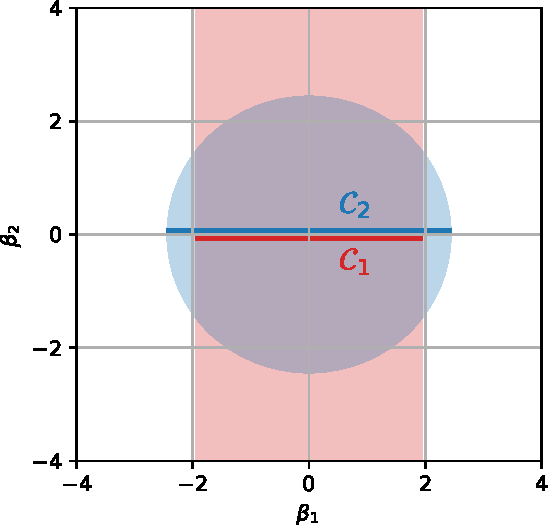
\includegraphics[width=\half]{E3p2_A.pdf} \caption{Confidence bands: single projection versus full vector.
            The two-dimensional vector $\beta$ is taken to be centered and to have unit covariance. Both highlighted areas
            have $95\%$ probability, but the band-shaped one has smaller projection on the $\beta_1$ axis. \label{3p2_f1}}
        
    \end{minipage}\halfspace
    \begin{minipage}{\half}
        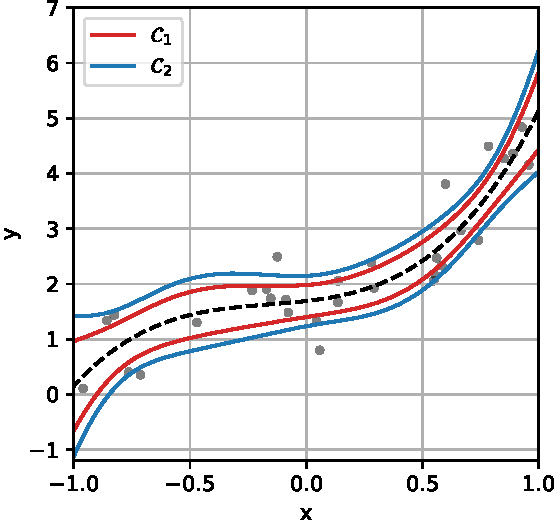
\includegraphics[width=\half]{E3p2_B.pdf} \caption{Confidence bands for a cubic univariate model. Values of $x$ have
            been drawn from a uniform distribution in $[-1, 1]$, and $y$ has been generated as $\beta^T x^{(3)} + \epsilon$,
            where $\beta$ is a centered, unit-covariance gaussian vector, $x^{(3)} \equiv (1, x, x^2, x^3)$ and $\epsilon$
            is a centered gaussian with variance equal to $0.25$. \label{3p2_f2}}
    \end{minipage}
\end{figure}